\documentclass[conference]{IEEEtran}
\IEEEoverridecommandlockouts
% The preceding line is only needed to identify funding in the first footnote. If that is unneeded, please comment it out.
\usepackage{cite}
\usepackage{amsmath,amssymb,amsfonts}
\usepackage{algorithmic}
\usepackage{graphicx}
\usepackage{textcomp}
\usepackage{xcolor}
\usepackage{caption}
\usepackage{subcaption}
\usepackage{subfiles}
\usepackage{siunitx}
\usepackage{gensymb}

\graphicspath{{\subfix{../images/}}}
\def\BibTeX{{\rm B\kern-.05em{\sc i\kern-.025em b}\kern-.08em
    T\kern-.1667em\lower.7ex\hbox{E}\kern-.125emX}}
\begin{document}

\title{Conference Paper Title*\\
{\footnotesize \textsuperscript{*}Note: Sub-titles are not captured in Xplore and
should not be used}
\thanks{Identify applicable funding agency here. If none, delete this.}
}

\author{\IEEEauthorblockN{1\textsuperscript{st} Given Name Surname}
\IEEEauthorblockA{\textit{dept. name of organization (of Aff.)} \\
\textit{name of organization (of Aff.)}\\
City, Country \\
email address or ORCID}
\and
\IEEEauthorblockN{2\textsuperscript{nd} Given Name Surname}
\IEEEauthorblockA{\textit{dept. name of organization (of Aff.)} \\
\textit{name of organization (of Aff.)}\\
City, Country \\
email address or ORCID}
\and
\IEEEauthorblockN{3\textsuperscript{rd} Given Name Surname}
\IEEEauthorblockA{\textit{dept. name of organization (of Aff.)} \\
\textit{name of organization (of Aff.)}\\
City, Country \\
email address or ORCID}
}

\maketitle

\begin{abstract}
With the growth of robotics, mobile robots are increasingly becoming a common aspect in key sectors of the economy. When compared to wheeled and tracked robots, legged robots present greater mobility and maneuverability, but less locomotion stability, which in turn demands more complex control systems. This paper aims to develop a quadruped robot capable of walking when teleoperated and assess its locomotion performance based on experiments. The first part of the methodology was dedicated to research and the definition of the robot's concept. The following stage involved the development of the robot's software, simulation, and, in parallel, the design, fabrication and assembly of the prototype. After both stages were done, the software was integrated into the prototype. After the integration stage, the locomotion experiments were conducted. Based on these experiments, it was possible to conclude that the robot was able to perform gaits of different sizes and walk in both plane and irregular terrains. Furthermore, it was observed that the body's rotation PID controller contributed to reducing the oscillation of the robot's body in both roll and pitch during walking in both terrains.
\end{abstract}

\begin{IEEEkeywords}
Quadruped robot; Locomotion; Control.
\end{IEEEkeywords}

\section{Introduction}
Com o avanço da robótica, robôs móveis estão cada vez mais ganhando espaço em setores chave da economia como o comercial, industrial e militar. Os robôs terrestres que se locomovem com pernas têm se mostrado mais eficientes para se locomover em terrenos irregulares, inclinados e escorregadios, e também para superar obstáculos \cite{X.134}. Quando comparados com robôs com rodas, robôs com pernas ainda possuem melhor mobilidade e manobrabilidade em ambientes complexos, o que possibilita transitar por caminhos não necessariamente contínuos. Entre os robôs com pernas, os quadrúpedes vêm ganhando destaque por apresentarem maior estabilidade e uma estrutura mais simples quando comparados aos bípedes e hexápodes \cite{Shi2021}.

O uso de uma plataforma com quatro pernas requer um sistema de locomoção robusto que envolve o controle de equilíbrio da plataforma, o controle das juntas do robô e o planejamento de marchas. Para poder aplicar todos esses conceitos e desenvolver aplicações reais com robôs quadrúpedes, é fundamental estudar sua estrutura física, os tipos de marcha que eles podem realizar e os métodos de controle de locomoção que são utilizados nesses robôs.

O objetivo deste trabalho é desenvolver um sistema robótico do tipo quadrúpede capaz de se locomover de forma estável quando teleoperado. Serão estudados aspectos construtivos, de locomoção e de controle desse tipo robô. Além disso, será projetado um protótipo que será simulado e fabricado, a fim de testar os algoritmos de locomoção não apenas em um ambiente virtual, mas também na prática. Por fim, serão realizados experimentos de performance de locomoção com o protótipo físico, os quais analisarão a estabilidade do robô em ambientes de terreno plano e irregular.

A seção \ref{sec:the_quadruped_robot} tratará dos conceitos estudados para o desenvolvimento do robô. A seção \ref{sec:methodology} explicará a metodologia utilizada durante o projeto. Na seção \ref{sec:the_caramel}, será apresentado o Caramelo, o robô desenvolvido para essa pesquisa. A seção \ref{sec:results} apresentará os resultados dos testes e experimentos realizados, ao passo que a seção \ref{sec:conclusion}, as conclusões feitas a partir dos resultados. Por fim, a seção \ref{sec:final_points} apresentará as considerações finais e as sugestões dos autores para trabalhos futuros.


\section{O Robô Quadrúpede}

O robô quadrúpede é um sistema robótico móvel que se locomove com a ajuda de pernas. Quando comparado a robôs terrestres que utilizam outros meios de locomoção --- como rodas ou esteiras ---, ele apresenta diversas particularidades que lhes confere muitas vantagens quanto à mobilidade, robustez a diferentes terrenos e superação de obstáculos \cite{Biswal2021}. Robôs com rodas e esteiras conseguem navegar pelo espaço, desde que haja um caminho contínuo entre os pontos de origem e de destino. Robôs com pernas, por outro lado, são capazes de escolher os melhores pontos no terreno para apoiar suas patas, o que permite uma navegação em caminhos discretos (com obstáculos de grande inclinação e variação de altura) \cite{Yao2021}. Essa capacidade de se adaptar a terrenos desnivelados favorece sua aplicação em setores  industrial e militar, atuando em missões de inspeção e de resgate. Por outro lado, esse tipo de robô apresenta menor estabilidade de locomoção e, por consequência, maior complexidade de controle.

Robôs com pernas também apresentam diversas diferenças entre si, majoritariamente ligadas à quantidade de pernas que possuem. A quantidade de pernas de um robô está diretamente relacionada a sua estabilidade, capacidade de locomoção e eficiência. Os bípedes possuem baixa estabilidade, visto que se apoiam em apenas uma perna para poderem andar. Aqueles com múltiplas pernas (mais de quatro) possuem maior estabilidade, visto que conseguem manter pelo menos três pontos de apoio no solo enquanto realizam um passo. No entanto, cada perna representa um conjunto adicional de juntas e atuadores, diminuindo a eficiência do sistema como um todo. Os quadrúpedes conseguem unir vantagens desses dois tipos ao apresentar um balanço entre estabilidade e eficiência. Eles possuem uma estabilidade passiva quando estáticos, pois se apoiam em quatro pontos. Além disso, também são capazes de navegar de forma estável em baixas velocidades, movendo uma perna por vez enquanto as outras três permanecem no solo. Isso elimina a redundância presente nos robôs com múltiplas pernas, aumentando sua eficiência \cite{Yao2021}.

\subsection{Estrutura e design}
Pelo fato de robôs quadrúpedes terem se tornado um grande foco de pesquisa nos últimos anos, diferentes \textit{designs} já foram pesquisados. Esses \textit{designs} se distinguem quanto à estrutura, configuração de pernas e o número de graus de liberdade (GDL) por perna.

Um dos tipos de estrutura existente é a de tipo mamífero. A estrutura tipo mamífero tem esse nome devido a sua semelhança com a postura de quadrúpedes, como cachorros e cavalos. Kitano \textit{et al.}, em \cite{Kitano2016}, analisa dois tipos diferentes de estruturas de robôs quadrúpedes: a do tipo mamífero (figura \ref{fig:robots_structures_b}) e a do tipo \textit{sprawling} (figura \ref{fig:robots_structures_c}). Segundo sua análise, a primeira permite alcançar maiores velocidades por possuir duas juntas no plano sagital. Além disso, ela também apresenta maior eficiência, pois os atuadores requerem menos torque para sustentar o robô: sua estrutura mais compacta diminui o braço de alavanca sobre o qual a força peso do robô atua. Essa estrutura também favorece a navegação em ambientes estreitos, onde um robô do tipo \textit{sprawling}, por exemplo, teria dificuldades de acessar.

\begin{figure}[htbp]
    \centering
    \begin{subfigure}[htbp]{0.23\textwidth}
        \centering
        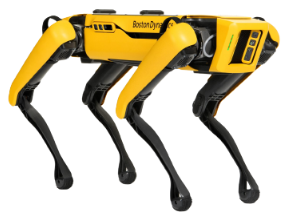
\includegraphics[width=0.9\textwidth]{Spot.png}
        \caption{Spot.}
        \label{fig:robots_structures_b}
    \end{subfigure}
    \begin{subfigure}[htbp]{0.23\textwidth}
        \centering
        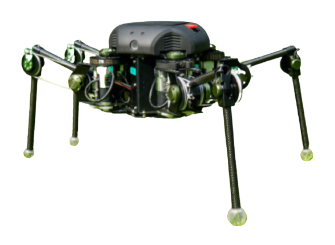
\includegraphics[width=1.0\textwidth]{Titan.png}
        \caption{TITAN-XIII.}
        \label{fig:robots_structures_c}
    \end{subfigure}
    \centering
    \caption{Exemplos de robôs com estruturas do tipo mamífero e \textit{sprawling}.}
    Fonte: Adaptado de  \cite{Kitano2016} e \cite{SpotImg1}.
    \label{fig:robots_structures}
\end{figure}

Os robôs quadrúpedes que utilizam essa estrutura também se diferenciam quanto à configuração das pernas. As duas configurações mais utilizadas podem ser vistas na figura \ref{fig:joint_configurations}. Robôs como o \textit{Spot}, \textit{MIT Cheetah} e \textit{Stanford Pupper} utilizam a configuração \textit{full-elbow}, enquanto outros como o \textit{ANYmal}, \textit{StarlETH} e \textit{BigDog} adotam a configuração \textit{elbow-knee}. Yao \textit{et al.}, em \cite{Yao2021}, acreditam que a configuração \textit{elbow-knee} possibilita maior estabilidade, mas as características de movimento da configuração \textit{full-elbow} podem ser superiores.

\begin{figure}[htbp]
  \centering
  \begin{subfigure}[htbp]{0.24\textwidth}
    \centering
    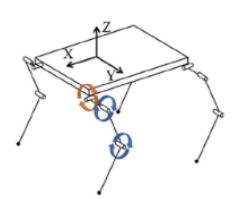
\includegraphics[width=1.0\textwidth]{full_elbow.png}
    \caption{\textit{full-elbow}.}
    \label{fig:joint_configurations_a}
  \end{subfigure}
  \begin{subfigure}[htbp]{0.24\textwidth}
      \centering
      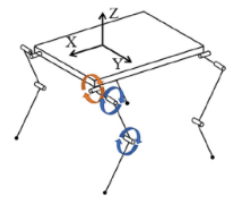
\includegraphics[width=1.0\textwidth]{elbow_knee.png}
      \caption{\textit{elbow-knee}.}
      \label{fig:joint_configurations_d}
  \end{subfigure}

  \caption{Tipos de configuração de pernas para robôs com estrutura tipo mamífero.}
  Fonte: Adaptado de \cite{Yao2021}.
  \label{fig:joint_configurations}
\end{figure}

O número de juntas nas pernas, que coincide com a quantidade de GDL do robô, também é um dos aspectos estudados sobre os quadrúpedes. A maioria apresenta 3 GDL por perna, o que é suficiente para que o robô consiga mover suas patas em três dimensões e realize diversos tipos de marchas. A fim de simplificar a estrutura e consequentemente o controle, alguns robôs utilizam apenas 2 GDL por perna, eliminando a junta no corpo que movimenta a perna no plano frontal. Outros robôs buscam performances mais semelhantes ao andar de animais reais, o que demanda maior flexibilidade de movimento, justificando o acréscimo de uma quarta junta. No entanto, como já mencionado, esse acréscimo aumenta a complexidade do controle e prejudica a eficiência. Essa perda de eficiência se dá porque a maior quantidade de atuadores resulta em um maior consumo de energia e em uma maior quantidade de massa.

A massa do robô quadrúpede deve ser a menor possível. Quanto mais leve for o sistema, menos torque será demandado dos motores e, consequentemente, maior sua eficiência. Além disso, a distribuição de massa do robô também é um aspecto muito importante. A massa deve ser localizada majoritariamente no corpo, enquanto as pernas devem possuir baixa inércia. Isso permite que elas se movam rapidamente sem alterar, de forma significativa, o centro de gravidade do robô, o que aumenta a estabilidade e requer menos complexidade de controle. Possuir baixa inércia significa possuir baixa massa. Por outro lado, as pernas devem ser resistentes o suficiente para suportar o peso do robô, além dos distúrbios causados pelo impacto das patas com o chão, o que pode demandar um aumento de massa nas pernas. Portanto, um equilíbrio entre massa e resistência deve ser buscado ao mesmo tempo em que deve-se buscar diminuir a massa total do sistema \cite{Zhong2019}.

\subsection{Movimentação por marchas}
Robôs quadrúpedes se movimentam conforme uma sequência de movimentos coordenados de suas pernas que compõem uma marcha. Uma marcha é definida pelo tempo e local de colocação e levantamento de cada pata, coordenado com o movimento do corpo em seus seis graus de liberdade, para mover o corpo de um lugar para outro  \cite{Song1989}.

A marcha é um aspecto fundamental para garantir que um robô com pernas caminhe de forma eficiente e estável, especialmente em terrenos irregulares \cite{X.129}. Para tanto, é necessário levar em consideração suas etapas e, consequentemente, seu tipo.

Marchas são divididas em duas etapas: \textit{stance} e \textit{swing}. Durante a fase \textit{stance}, as pernas estão no solo e impulsionam o robô para frente. Na etapa de \textit{swing}, as pernas são erguidas para deslocar a pata até o próximo ponto de apoio. É importante ressaltar que as fases de \textit{stance} e \textit{swing} não ocorrem em todas as pernas simultaneamente. A depender do tipo de marcha, algumas pernas podem estar em \textit{swing} enquanto outras estarão em \textit{stance}.

O \textit{trot} é um tipo de marcha muito utilizado por robôs quadrúpedes, devido a sua simplicidade e eficiência. Este tipo de marcha é periódico e simétrico. Marchas periódicas são caracterizadas pela repetição contínua dos mesmos movimentos nos mesmos instantes, dentro de um ciclo de locomoção \cite{de2006quadrupedal}. Já a simetria é uma característica de marchas que movimentam um par de pernas em conjunto, saindo e voltando para o solo de forma sincronizada. No \textit{trot}, as pernas diagonais se movimentam em pares, e quando um par está na etapa de \textit{swing}, o outro está na etapa de \textit{stance}. Outra característica da marcha \textit{trot} é que ela pode ser contínua ou descontínua. Uma marcha contínua mantém o corpo do robô em movimento constante, enquanto que a descontínua submete o corpo a um movimento intermitente \cite{de2006quadrupedal}. Portanto, quando a marcha \textit{trot} é contínua, as pernas em \textit{stance}, além de sustentarem o robô, deslocam o corpo na direção do movimento, o que exige maior capacidade de controle. Em contrapartida, quando ela é descontínua, o corpo fica estático, esperando as pernas em \textit{swing} terminarem o movimento para, então, ser deslocado, tão logo as quatro pernas estejam no solo.

\subsection{Controle de locomoção}

Todo o controle de locomoção do robô é realizado pelo planejador de marchas. Ele é o responsável por enviar os comandos para que as pernas se movam para os locais desejados, no momento esperado. Logo, o planejador irá apenas ditar o ponto no espaço no qual cada pata do robô deve estar, em relação a um eixo de referência, cabendo ao sistema de controle executar o movimento. A seguir, serão discutidos dois itens fundamentais do sistema de controle de um robô quadrúpede: o modelo cinemático e as estratégias de controle.

% \subsubsection{Modelo cinemático}
% O modelo cinemático de um robô quadrúpede descreve a relação entre a posição de uma pata em três dimensões com a rotação de cada junta da sua respectiva perna. Como todas as pernas do robô são iguais, pode-se formular as relações de apenas uma perna e replicá-la quatro vezes, acrescentando as devidas translações e rotações, para obter o modelo cinemático de todo o sistema.

% O modelo cinemático pode ser usado para resolver dois problemas: a cinemática direta e a cinemática inversa. A cinemática direta fornece a posição de uma pata em $(x, y, z)$ em função dos ângulos das juntas, enquanto que a cinemática inversa fornece os ângulos das juntas correspondentes a uma posição da pata no espaço tridimensional. Esses dois problemas são complementares, sendo a saída de um a entrada do outro, e vice-versa. A partir da cinemática inversa, o robô consegue determinar quanto deve rotacionar seus atuadores para mover a pata a alguma distância nas direções $(x, y, z)$. Com a cinemática direta, é possível saber se a pata de fato chegou na posição em que ele deveria estar. Portanto, ambos são muito importantes para o controle de locomoção do robô.

\subsubsection{Estratégias de controle}
A locomoção de robôs quadrúpedes, em geral, segue uma sequência de passos. Raibert propõe em \cite{Raibert1986} um método de controle baseado em três etapas: controle de salto, controle de velocidade e controle de postura do corpo. Essa estratégia de controle foi utilizada para controlar robôs com uma, duas, e quatro pernas (o controle de salto se justifica porque robôs com apenas uma perna só podem ser locomover saltando). Sua premissa básica era a de que apenas uma perna estaria em \textit{stance} ou em \textit{swing} por vez. Para que robôs com mais de duas pernas satisfaçam essa premissa, foi proposto o conceito de pernas virtuais. Isto é, um conjunto de pernas deve realizar igual comportamento quando em \textit{swing} e \textit{stance} e as fases de \textit{swing} e \textit{stance} de cada conjunto devem ser alternadas. Esse conceito foi utilizado para embasar o uso de marchas simétricas e periódicas como o \textit{trot}.

Essa estratégia de controle em três etapas foi responsável por locomover robôs com pernas rígidas (apenas 2 GDL por perna, sendo uma junta rotativa e outra prismática) de maneira simples. No entanto, esses robôs apenas operavam no terreno plano e controlado do laboratório. A fim de possibilitar a operação de robôs com pernas em terrenos desnivelados e de difícil mobilidade, Raibert \textit{et al.} propôs um outro sistema de controle no seu trabalho sobre o \textit{BigDog} \cite{RAIBERT200810822}. O \textit{BigDog} é um robô quadrúpede com 4 GDL por perna movido por atuadores hidráulicos. Essa maior flexibilidade de movimentação das pernas permite controlar a locomoção do robô sem que este precise saltar, sendo possível, então, dividir o controle de locomoção em duas etapas principais: controle de \textit{stance} e controle de \textit{swing}. Como o nome sugere, o controlador de \textit{stance} é o responsável por controlar o comportamento das pernas na fase de \textit{stance}, enquanto o controlador de \textit{swing} é o responsável por controlar as pernas em \textit{swing}. Vale lembrar que durante a marcha, algumas pernas podem estar na etapa de \textit{swing} enquanto outras estão na etapa de \textit{stance}, o que significa que esses controladores ora assumem o comando de um par de pernas, ora de outro (essa troca não necessariamente se dá em pares, porém isso é válido para marchas simétricas como o \textit{trot}). Quem define o momento em que cada controlador assume o controle de uma determinada perna é o planejador de marchas.

O modo como cada perna se comporta durante as etapas de \textit{stance} e \textit{swing} pode variar em diversos aspectos, mas ainda é possível elencar semelhanças gerais. No início da etapa de \textit{swing}, calcula-se o local do próximo ponto de apoio das patas com base na velocidade desejada para o robô e uma trajetória de passo até esse ponto. Essa trajetória pode ter o formato de uma curva senoidal \cite{X.118}, triangular \cite{StanfordPupper}, de Bezier \cite{HackadayQuadruped}, cicloidal \cite{Shi2021} \cite{X.58}, entre outras. Uma consideração que pode ser feita a fim de simplificar o sistema de controle é de que a movimentação das pernas durante a fase de \textit{swing} não interfere no movimento do corpo do robô. Para que isto seja válido, é necessário controlar a força com que a pata toca o solo, a fim de diminuir os distúrbios causados no corpo do robô. A força de contato entre as patas e o solo é um ponto-chave para a estabilidade do quadrúpede \cite{X.118}. Nesse sentido, a trajetória cicloidal ganha destaque por conta de sua primeira derivada nula no momento em que se aproxima do seu ponto mínimo.

Já na fase de \textit{stance}, as pernas devem manter o robô em equilíbrio, além de deslocar o corpo na direção desejada de locomoção. Para isso, alguns robôs utilizam trajetórias para as patas com um formato pré-determinado, assim como na fase de \textit{swing}, não necessariamente repetindo o mesmo formato de curva \cite{X.118, X.58}. Além disso, controladores de equilíbrio também podem ser implementados nessa etapa. Esses controladores visam estabilizar os ângulos de \textit{pitch} e \textit{roll} do robô \cite{Shi2021, StanfordPupper, HackadayQuadruped, Notspot} ou ainda outros graus de liberdade \cite{X.134, Chen2020140736, Zhang2016284}. Eles podem controlar diretamente a angulação do corpo do robô (com o auxílio de um sensor inercial) e/ou a força de contato com o solo em cada perna, por exemplo. No entanto, alguns trabalhos se baseiam apenas no controle individual de cada junta para manter o robô em equilíbrio, o que é uma abordagem mais simples, mas que pode falhar, especialmente em terrenos irregulares.

\section{Metodologia}
Para o desenvolvimento do projeto, foi seguida uma metodologia própria composta por três etapas sequenciais: fundamentação, desenvolvimento e resultados e análises. A seguir, serão detalhadas cada uma dessas etapas.

  \subsection{Fundamentação}
  Com o intuito de buscar referências para o projeto, foi utilizado o método \textit{Bibliographic and Literary Review Method} (\textit{BiLi}), que consiste em um método de busca iterativa de artigos, guiada por análises estatísticas das palavras-chave e da rede de co-citação entre os trabalhos encontrados \cite{bili}. Em seguida, foi realizado um \textit{benchmarking} de projetos \textit{open source} de robôs quadrúpedes para auxiliar na definição do conceito do robô que será projetado e prototipado.
  
  \subsection{Desenvolvimento}
  Durante esta etapa, houve o desenvolvimento do robô propriamente dito. Foram criadas duas frentes de trabalho que ocorreram em paralelo: a implementação e simulação dos algoritmos em ambiente computacional, e a criação do \textit{design} junto à prototipação do robô.

  Durante a implementação dos algoritmos na simulação, foram elaborados, primeiramente, o diagrama de blocos do sistema e a arquitetura de \textit{software} do controlador. A partir disso, os algoritmos de cinemática e controle foram implementados e testados na simulação. Para auxiliar o desenvolvimento do projeto, algumas ferramentas de \textit{softwares} foram utilizadas, como o \textit{ROS2 Humble} e o simulador \textit{Gazebo}.

  Em paralelo ao desenvolvimento do \textit{software}, foi realizado o \textit{design} e a prototipação do robô através da elaboração dos desenhos mecânicos e do projeto eletroeletrônico. Esta etapa incluiu também a impressão 3D das partes mecânicas, o teste dos atuadores e sensores e a configuração da comunicação entre a central de processamento e os atuadores, culminando na montagem física do protótipo. Durante essa etapa, o \textit{software} \textit{OnShape} foi utilizado para a modelagem 3D do robô e o \textit{QElectroTech}, para o projeto eletroeletrônico.

  Após essas duas etapas, foi possível realizar a integração dos algoritmos no protótipo físico. Ao final da integração, o protótipo já estava funcional e pronto para a fase de testes.

  \subsection{Resultados e análises}
  \label{sec:method_results_analysis}
  Durante a etapa de resultados e análises, foram feitos testes para fins de avaliação do funcionamento e da performance de locomoção do robô. Eles foram divididos em dois grupos: testes preliminares e experimentos de locomoção. 
  
  Os testes preliminares objetivaram testar três funcionalidades básicas do robô: a movimentação do corpo com base no modelo cinemático, o controle de angulação do corpo e a execução da trajetória do passo. As duas primeiras funcionalidades foram avaliadas de forma qualitativa e a última de forma estatística. Esses testes são importantes porque ambas as funcionalidades são utilizadas nos experimentos de locomoção e influenciam diretamente no comportamento do robô. 

  Os experimentos de locomoção foram realizados a fim de avaliar a locomoção do robô em terrenos planos e irregulares. Para isso, foi verificada a capacidade do robô de seguir um comando de velocidade pré-estabelecido e de manter a orientação do seu corpo estável em $0°$ nos ângulos de \textit{roll} e \textit{pitch}. A análise dos dados se deu mediante métodos estatísticos. O teste de Shapiro-Wilk \cite{leotti2005comparaccao} foi aplicado para verificar a normalidade dos dados. Caso eles se assemelhassem a uma distribuição normal, a Análise de Variância (ANOVA) \cite{cano2012six} poderia ser utilizada para verificar se os dados analisados são estatisticamente semelhantes ou não.

  O primeiro teste preliminar consistiu em enviar comandos de posição e orientação para o corpo do robô individualmente em cada um dos eixos ($x, y, z$, \textit{roll}, \textit{pitch} e \textit{yaw}) e observar seu comportamento. O segundo teste teve o objetivo de verificar a resposta do controle de angulação do robô a diferentes valores de rotações desejadas. Para isso, foram aplicados sinais degrau nos \textit{setpoints} de angulação em $roll$ e em $pitch$, simultaneamente, e as respostas do sistema foram analisadas de forma gráfica.
  
  O terceiro teste preliminar consistiu em mover uma das patas por uma trajetória cicloidal feita pelo planejador de trajetórias. Para isso, o corpo do robô foi apoiado em um suporte elevado, de modo que as patas não tocassem o chão, diminuindo a carga sobre os motores. O objetivo principal deste teste foi verificar se o sistema de controle do robô era capaz de responder de forma coerente aos comandos enviados pelo planejador de marchas numa situação mais próxima da ideal (sem carga). As trajetórias foram calculadas considerando a altura de passo $0,05 m$, período de $0,5 s$ e uma resolução de $25$ pontos distribuídos de forma homogênea ($P_T = P_N = 1,0$). Foram feitos dois tipos de testes, variando as distâncias que a pata deve percorrer nas coordenadas $x$ e $y$, e para cada teste foram coletadas 30 amostras. Desta forma, foi possível realizar uma análise estatística, assim como feito com os experimentos de locomoção.
  
  Os experimentos de locomoção foram realizados em dois tipos de terreno: um chão de cimento plano (figura \ref{fig:terreno_plano}) e um terreno irregular formado por pequenas pedras soltas (figura \ref{fig:terreno_irregular}). Estes experimentos consistiram em enviar um comando de velocidade constante para frente de $0,05 m/s$ e medir o tempo que o robô precisou para percorrer $1,5 m$. Assim, foi possível inferir a velocidade média e compará-la com o comando enviado. Além disso, visando avaliar a contribuição do controle de angulação do robô para sua estabilidade, metade dos experimentos foram realizados com esta funcionalidade ativa e a outra não. A estabilidade do robô foi mensurada por meio da oscilação máxima do corpo do robô nos ângulos de \textit{roll} e \textit{pitch}. A trajetória utilizada para o passo possui as mesmas especificações utilizadas no terceiro teste preliminar, exceto pelos parâmetros de disposição dos pontos, cujos valores adotados foram $P_T = 0,66$ e $P_N = 0,33$. Os experimentos foram organizados em quatro combinações de testes, variando o tipo do terreno e o uso, ou não, do controle de angulação. Para cada um dos 4 testes, foram coletadas 10 amostras.

  \begin{figure}[htbp]
    \centering
    \begin{subfigure}[htbp]{0.24\textwidth}
      \centering
      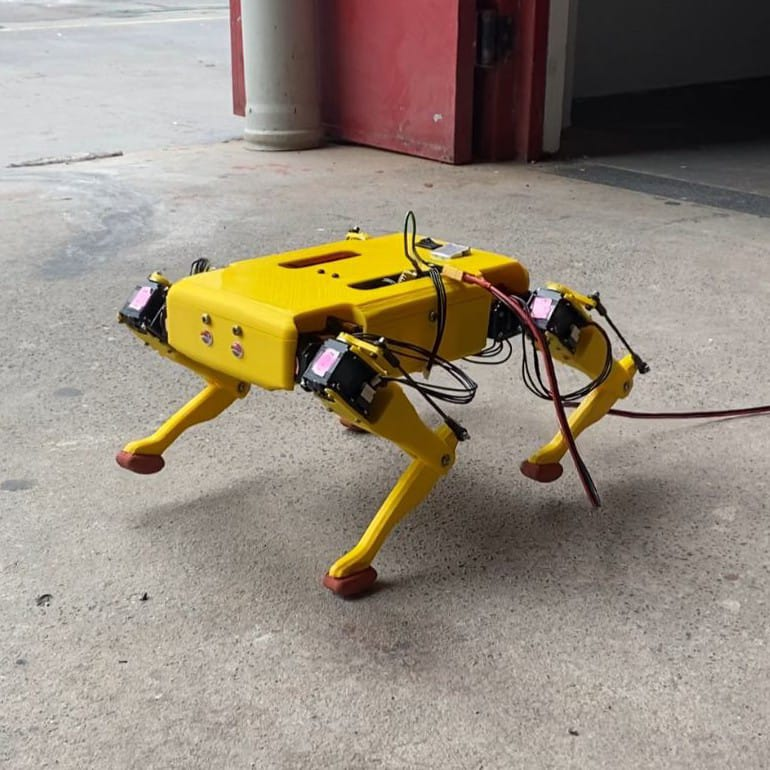
\includegraphics[width=1.0\textwidth]{terreno_plano.jpeg}
      \caption{Plano.}
      \label{fig:terreno_plano}
    \end{subfigure}
    \begin{subfigure}[htbp]{0.24\textwidth}
      \centering
      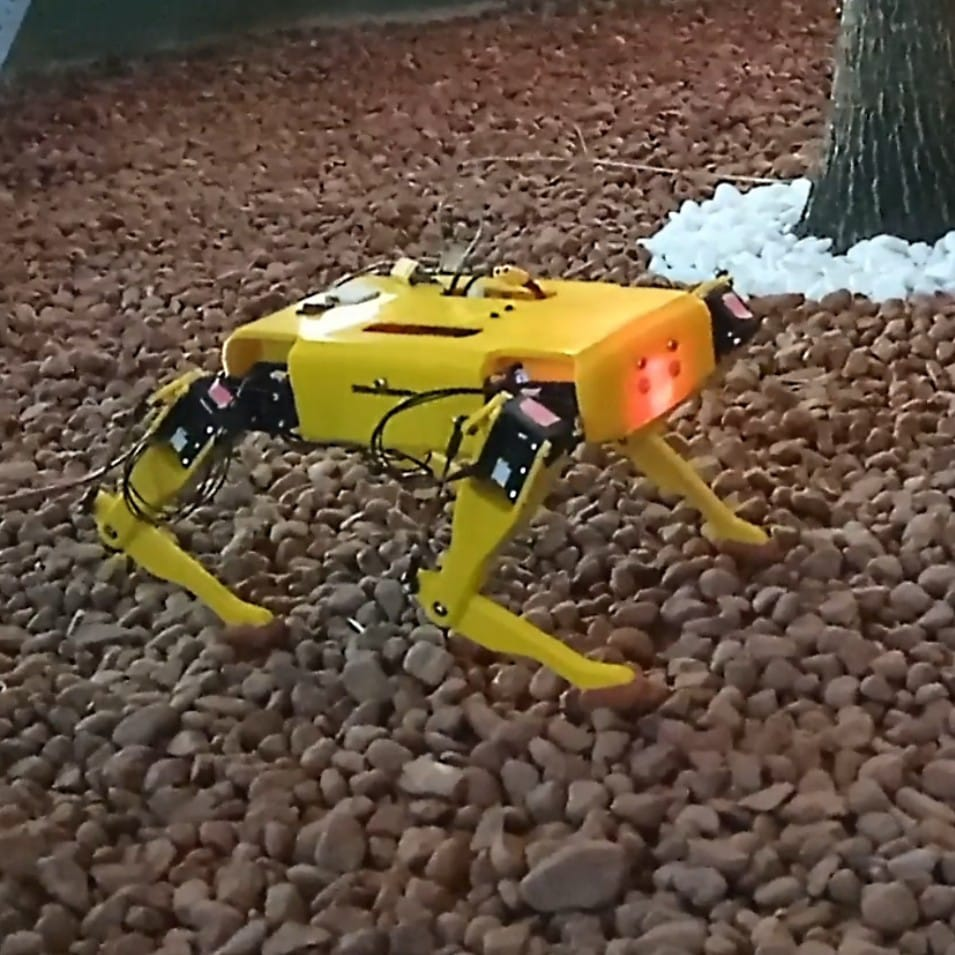
\includegraphics[width=1.0\textwidth]{terreno_irregular.jpeg}
      \caption{Irregular.}
      \label{fig:terreno_irregular}
    \end{subfigure}
    \vfill
    \caption{Terrenos dos testes.}
    Fonte: autores.
    \label{fig:terrenos}
  \end{figure}

\section{O Robô Caramelo}

Baseado nos conceitos apresentados, foi projetado, simulado e desenvolvido um robô quadrúpede nomeado de Caramelo (figuras \ref{fig:terrenos}, \ref{fig:caramel_body} e \ref{fig:moving_body}). Caramelo é um robô quadrúpede de pequeno porte voltado para pesquisa e educação. Seu \textit{hardware} foi modelado inteiramente pela equipe e impresso com impressora 3D no material ABS. Os atuadores do robô são servomotores do modelo \textit{dynamixel} MX-28 e sua central de processamento é composta por uma \textit{RaspberryPi} 4. Além disso, ele conta com um sensor inercial modelo MPU6050, que está instalado no corpo do robô. Este sensor contém um giroscópio e um acelerômetro, o que permite obter a aceleração linear, a velocidade angular e a orientação do corpo do robô. Todo o \textit{software} foi desenvolvido com o \textit{Robot Operating System 2 Humble} (\textit{ROS2}) \cite{ROS2Humble}, que consiste em um \textit{framework} de robótica \textit{open source} com vários recursos disponíveis para facilitar o desenvolvimento de sistemas robóticos.

A estrutura do Caramelo é do tipo mamífero e a configuração das pernas é a \textit{full-elbow}. Além disso, possui 3 GDL por perna, o que permite uma grande liberdade de movimentação para as patas. Seu \textit{design} foi pensado para favorecer o balanço de massas entre o corpo e as pernas do robô, ou seja, a maior parte da massa se encontra no corpo ou próxima a ele. Os componentes eletrônicos internos, que abrangem sensores, unidades de processamento e a interface de comunicação com os atuadores, foram dispostos de forma simétrica, a fim de manter o centro de massa o mais próximo do centro do corpo. Os motores (componentes que contribuem com a maior massa para o sistema) foram dispostos o mais próximo possível do corpo. Um destaque para o motor que atua na junta da tíbia foi sua instalação na parte superior do fêmur, com o objetivo de diminuir o momento de inércia da perna. Essa escolha demandou a adição de um sistema de transmissão entre o eixo do motor e a tíbia, formado por uma haste rígida de metal com uma junta esférica em cada extremidade.

A locomoção do Caramelo foi desenvolvida baseada nas marchas periódicas e simétricas. Dessa forma, foi adotada a marcha \textit{trot} como a marcha principal do robô. Embora sua estrutura permita a realização de muitos outros tipos de marcha, neste trabalho, foi considerada apenas o \textit{trot}, devido a sua simplicidade e eficiência. Com o objetivo de diminuir a complexidade do controle de locomoção, foi adotada uma marcha descontínua, ou seja, o corpo do robô se desloca apenas quando todas as patas estão no solo. A sequência de etapas da marcha do Caramelo pode ser vista na figura \ref{fig:trot_pattern}, cujas áreas em branco representam a etapa de \textit{swing} e as em cinza a de \textit{stance}. É possível perceber que sempre o mesmo par de pernas diagonais se move no mesmo instante. Entre duas etapas consecutivas de \textit{swing}, há um momento em que todas as patas estão em \textit{stance}, que é quanto o corpo do robô é deslocado no sentido desejado de locomoção.

\begin{figure}[htbp]
  \centering
  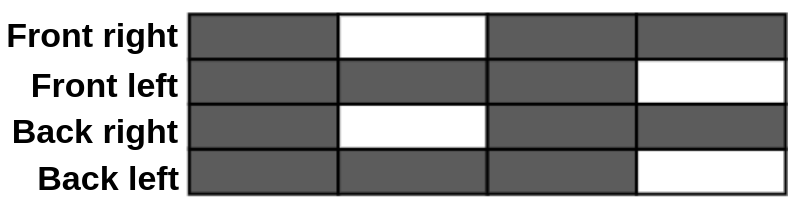
\includegraphics[width=0.45\textwidth]{trot_pattern.png}
  \vfill
  \caption{Padrão de movimentação da marcha para cada perna.}
  Fonte: autores.
  \label{fig:trot_pattern}
\end{figure}

O sistema de controle do robô é composto por dois subsistemas principais: os controladores individuais de cada junta e os controladores da angulação do corpo do robô. Os controladores das juntas são os próprios controladores PID embarcados nos motores \textit{dynamixel}. Foi utilizada a interface de controle de posição com o atuador, de forma que o \textit{setpoint} de controle enviado para cada motor é o ângulo em radianos para o qual ele deve rotacionar. O modelo cinemático do robô, apresentado na seção \ref{sec:detail_inv_kinematics}, é o responsável por mapear não apenas a posição tridimensional de cada pata com a angulação de cada junta, mas também a posição do corpo em seis dimensões: translação e rotação em $(x, y, z)$. Dessa forma, é possível controlar cada pata e o corpo do robô ao mesmo tempo de forma independente. Os controladores de angulação do corpo são dois controladores PID em paralelo, responsáveis por controlar o ângulo de \textit{pitch} (rotação em $y$) e o de \textit{roll} (rotação em $x$).

O planejador de marchas é o responsável por controlar cada pata do robô e, por consequência, o corpo. Ele calcula a trajetória que cada pata deve realizar, com base nas etapas de \textit{stance} e \textit{swing}, e envia o próximo ponto em que cada pata deve estar, a uma frequência de $\SI{50}{\hertz}$. Essa frequência foi definida por ser a maior que o sistema de processamento do robô foi capaz de suportar e por respeitar o teorema Nyquist, que indica que, nesse caso, a frequência deve ser maior do que $\SI{4}{\hertz}$ --- já que o período do passo é $0.5 s$. Além disso, o planejador de marchas também considera o esforço de controle enviado pelos controladores de angulação, de modo a manter o corpo do robô em $0^{\circ}$ a todo momento.

A seguir, será apresentado o desenvolvimento do modelo cinemático, dos controladores de angulação e da trajetória que cada pata realiza na etapa de \textit{swing}.

\subsection{Kinematic model}
\label{sec:detail_inv_kinematics}

The kinematic model of a quadruped robot describes the relationship between the position of the paw in the three-dimensional space with the rotation of each joint of its corresponding leg. This model is used to solve the forward kinematics, which provides the position $(x, y, z)$ of the paw as a function of leg joint angles, and inverse kinematics, responsible for giving the rotation of each joint to achieve the desired paw's position in space. Moreover, this model can be extended to encompass the kinematics of the quadruped's body.

The \textit{tf2} package, an available \textit{ROS2} feature that can manage transformations between coordinate axes, was used to solve the robot's forward kinematics. The inverse kinematics, otherwise, have been done based on geometric analysis. The variables $\theta_1$, $\theta_2$ and $\theta_3$ express the angular position of each robot leg joint, and they can be calculated with the help of (\ref{eq:theta1}) to (\ref{eq:B}), as a function of the desired position $(x_{IK}, y_{IK}, z_{IK})$ for the paw and the lengths $L_1$, $L_2$ and $L_3$ (Fig. \ref{fig:caramel_tfs}).

% Como dito anteriormente, o modelo cinemático é utilizado para resolver a cinemática inversa e a cinemática direta do robô. Para a cinemática direta, foi utilizado o pacote \textit{tf2}, um recurso disponível no \textit{ROS2} que facilita o gerenciamento de transformações entre eixos de coordenadas. A cinemática inversa, por outro lado, foi feita com base em uma análise geométrica. As variáveis $\theta_1$, $\theta_2$ e $\theta_3$ expressam a posição angular de cada uma das juntas de uma perna do robô e são calculadas com auxílio das equações \ref{eq:theta1} a \ref{eq:B} em função da posição $(x_{IK}, y_{IK}, z_{IK})$ desejada para a pata e dos comprimentos $L_1$, $L_2$ e $L_3$ (figura \ref{fig:caramel_tfs}).
\begin{equation}
  \label{eq:theta1}
  \theta_1 = \arctan{(\frac{x_{IK}}{y_{IK}})} - \arctan{(\frac{L_1}{a})}
\end{equation}
\begin{equation}
  \label{eq:theta2}
  \theta_2 = \frac{\pi}{2} - \arctan{(\frac{a}{z_{IK}}}) - \arctan{(\frac{\sqrt{1-A^2}}{A})}
\end{equation}
\begin{equation}
  \label{eq:theta3}
  \theta_3 = \arctan(\frac{\sqrt{1-B^2}}{B})
\end{equation}
\begin{equation}
  \label{eq:a}
  a = \sqrt{x_{IK}^2+y_{IK}^2-L_1^2}
\end{equation}
\begin{equation}
  \label{eq:A}
  A =\frac{a^2+z^2+L_2^2-L_3^2}{2L_2\sqrt{a^2+z_{IK}^2}}
\end{equation}
\begin{equation}
  \label{eq:B}
  B = \frac{a^2+z_{IK}^2-L_2^2-L_3^2}{2L_2L_3}
\end{equation}

\begin{figure}[htbp]
  \centering
  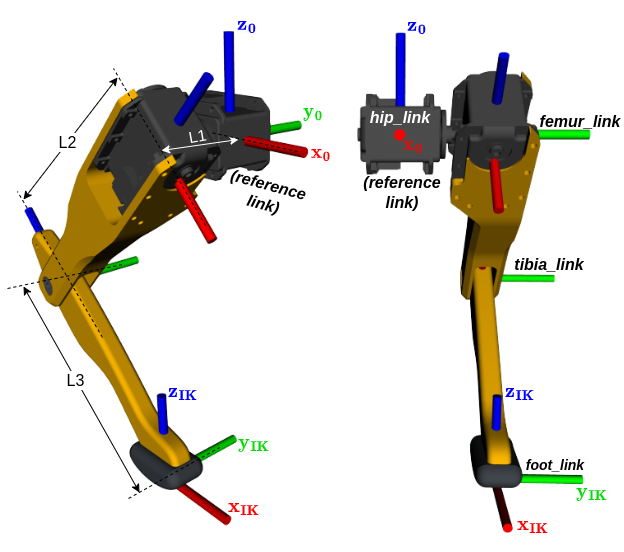
\includegraphics[width=0.4\textwidth]{caramel_tfs.png}
  
  \caption{Links from the robot leg.}
  \label{fig:caramel_tfs}
\end{figure}

These equations are useful for calculating only one paw's position but are insufficient to realize the robot's body kinematics. For that, a center frame called \textit{base\_link} (Fig. \ref{fig:caramel_body}) is taken as reference. The transformation matrix $T_M$ is created from the desired body translations $(x_c, y_c, z_c)$ and rotations $(\alpha, \beta, \gamma)$. The transformations $T_{FR}$, $T_{FL}$, $T_{BL}$ and $T_{BR}$ of each of the shoulders (\textit{hip\_links}) with respect to the \textit{base\_link} are also required.

% Essas equações são úteis para o cálculo da posição de uma única pata, mas são insuficientes para realizar a cinemática do corpo do robô. Desta forma, um \textit{frame} central, chamado de \textit{base\_link} (figura \ref{fig:caramel_body}), é utilizado como referência, e é criada uma matriz de transformação $T_M$ a partir das translações $(x_c, y_c, z_c)$ e rotações $(\alpha, \beta, \gamma)$ desejadas para o corpo, sendo possível controlar cada um dos 6 graus de liberdade. Para tanto, as transformações $T_{FR}$, $T_{FL}$, $T_{BL}$ e $T_{BR}$ de cada um dos ombros (\textit{hip\_links}) em relação ao \textit{base\_link} são necessárias.

% \begin{equation}
%   \label{eq:Tm}
%   T_M =
%   \begin{bmatrix}
%       &         &   & x_c \\
%       & R_{xyz} &   & y_c \\
%       &         &   & z_c \\
%     0 & 0       & 0 & 1
%   \end{bmatrix}
% \end{equation}
% \begin{equation}
%   \label{eq:Rxyz}
%   \begin{split}
%     R_{xyz} =
%     \begin{bmatrix}
%       1 & 0          & 0           \\
%       0 & \cos\alpha & -\sin\alpha \\
%       0 & \sin\alpha & \cos\alpha
%     \end{bmatrix}
%     \\.
%     \begin{bmatrix}
%       \cos\beta  & 0 & \sin\beta \\
%       0          & 1 & 0         \\
%       -\sin\beta & 0 & \cos\beta
%     \end{bmatrix}
%     \\.
%     \begin{bmatrix}
%       \cos\gamma & -\sin\gamma & 0 \\
%       \sin\gamma & \cos\gamma  & 0 \\
%       0          & 0           & 1
%     \end{bmatrix}
%   \end{split}
% \end{equation}

\begin{figure}[htbp]
  \centering
  \vspace{-0.75cm}
  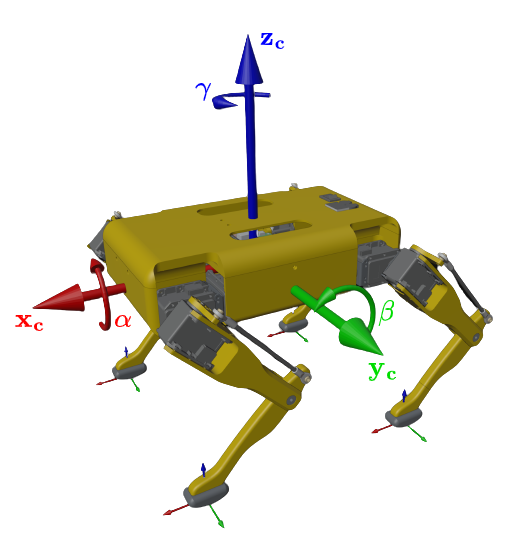
\includegraphics[width=0.35\textwidth]{caramel_body.drawio.png}
  
  \caption{Robot axes in resting position.}
  \label{fig:caramel_body}
\end{figure}

The calculation of joints angles of each robot's leg is then done using as input the $(x_{IK}, y_{IK}, z_{IK})$ values resulting from each of the transformations, according to (\ref{eq:xyzik}). The same calculation is done for the other legs, using $T_{FL}$, $T_{BL}$ and $T_{BR}$. In this way, inverse kinematics can compute the angulations $\theta_1$, $\theta_2$ e $\theta_3$ of each leg from the desired position of each paw and the desired translations and rotations of the body, making it possible to control it in each of the six degrees of freedom.

% O cálculo das angulações de cada perna então é feito utilizando como entrada os valores $(x_{IK}, y_{IK}, z_{IK})$ resultantes de cada uma das transformações, conforme (\ref{eq:xyzik}). O mesmo cálculo é feito para as demais pernas, utilizando  $T_{FL}$, $T_{BL}$ e $T_{BR}$. Desta forma, a cinemática inversa é capaz de computar as angulações  $\theta_1$, $\theta_2$ e $\theta_3$ de cada uma das pernas a partir da posição $(x, y, z)$ das patas em relação ao link central do robô e às translações $(x_c, y_c, z_c)$ e rotações $(\alpha, \beta, \gamma)$ desejadas para o corpo.

\begin{equation}
  \label{eq:xyzik}
  \begin{bmatrix}
    x_{IK} \\
    y_{IK} \\
    z_{IK} \\
    1
  \end{bmatrix}= (T_M.T_{FR})^{-1}.
  \begin{bmatrix}
    x \\
    y \\
    z \\
    1
  \end{bmatrix}
\end{equation}

% Desta forma, a cinemática inversa é capaz de computar as angulações  $\theta_1$, $\theta_2$ e $\theta_3$ de cada uma das pernas a partir da posição $(x, y, z)$ das patas em relação ao link central do robô e às translações $(x_c, y_c, z_c)$ e rotações $(\alpha, \beta, \gamma)$ desejadas para o corpo. Entretanto, em muitos casos, é mais conveniente realizar o cálculo dos ângulos passando como entrada as posições $(x, y, z)$ das patas em relação à sua posição \textit{default}, ou seja, a posição do seu \textit{foot\_link} quando o robô está em seu estado de repouso (figura \ref{fig:caramel_body}). Para isso, é possível realizar, previamente ao cálculo das angulações, mais uma transformação, desta vez do \textit{base\_link} para cada uma das posições \textit{default} das patas (equação \ref{eq:xyzik_foot}).
% \begin{equation}
%   \label{eq:xyzik_foot}
%   \begin{bmatrix}
%     x_{ik} \\
%     y_{ik} \\
%     z_{ik} \\
%     1
%   \end{bmatrix}= (T_M.T_{FR})^{-1}.
%   (F_{FR}.
%   \begin{bmatrix}
%     x \\
%     y \\
%     z \\
%     1
%   \end{bmatrix})
% \end{equation}

\subsection{Body rotation control}

Two identical PID controllers were employed to control the \textit{roll} and \textit{pitch} rotation of the robot body. They act independently, stabilizing the angulation in each axis simultaneously. Both controllers are identical and were implemented following the model shown in the block diagram in Fig. \ref{fig:pid}.

% Os controladores de angulação são dois controladores PID em paralelo, responsáveis por controlar a rotação de \textit{roll} e \textit{pitch} do corpo do robô. Eles atuam de forma independente, controlando a rotação do corpo em ambos os eixos simultaneamente. Ambos os controladores são iguais e foram implementados seguindo o modelo apresentado no diagrama de blocos da figura \ref{fig:pid}.
\begin{figure}[htbp]
  \centering
  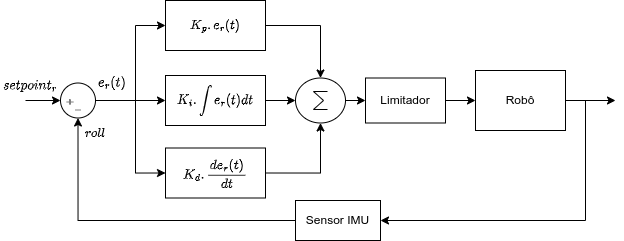
\includegraphics[width=0.48\textwidth]{PID.drawio.png}
  \caption{Designed PID controller.}
  \label{fig:pid}
\end{figure}

The IMU sensor is responsible for measuring the rotation of the robot body, enabling the feedback of the system outputs. The limiter was added to avoid sending values that exceed the rotation limits of the robot joints. The control efforts are sent to the gait planner, which, in turn, sends the movement commands to the joint controllers.

% O IMU é o sensor responsável por medir a rotação do corpo do robô, possibilitando a realimentação das saídas do sistema. O limitador foi adicionado para evitar que sejam enviados valores que extrapolam os limites de rotação das juntas do robô. Os esforços de controle são enviados para o planejador de marchas que, por sua vez, envia os comandos de movimentação para os controladores das juntas.

\subsection{Planejador de trajetória}

O planejador de trajetória é responsável por calcular a trajetória que cada pata deve realizar, tanto na fase de \textit{stance} quanto na fase de \textit{swing}. Para o Caramelo, a trajetória é uma curva cicloidal em ambas as etapas. Como apresentado em \cite{Shi2021}, uma curva cicloidal pode ser definida no espaço tridimensional entre os pontos $(x_o, y_o, z_o)$ e $(x_f, y_f, z_f)$ em função do tempo $t$ pelas equações (\ref{eq:traj_x}) a (\ref{eq:traj_k}), sendo $H$ a altura do passo e $T$ o período.
\begin{equation}
  x = (x_f - x_o) \frac{K - \sin{(K)}}{2 \pi} + x_o
  \label{eq:traj_x}
\end{equation}
\begin{equation}
  y = (y_f - y_o) \frac{K - \sin{(K)}}{2 \pi} + y_o
  \label{eq:traj_y}
\end{equation}
\begin{equation}
  z = H \frac{1 - \cos{(K)}}{2} + z_o
  \label{eq:traj_z}
\end{equation}
\begin{equation}
  K = \frac{2 \pi t}{T}
  \label{eq:traj_k}
\end{equation}

O gráfico de uma curva cicloidal no espaço 3D pode ser vista na figura \ref{fig:traj_space}. A mesma trajetória é ilustrada na figura \ref{fig:traj_time} em função do tempo. É possível perceber que a curva possui a primeira derivada nula no momento em que a pata toca o solo, o que é favorável ao controle de malha aberta, uma vez que quanto mais suave a aterrissagem, menos distúrbios são causados no sistema.

\begin{figure*}[h]
    \centering
    \begin{subfigure}[t]{0.32\textwidth}
      \centering
      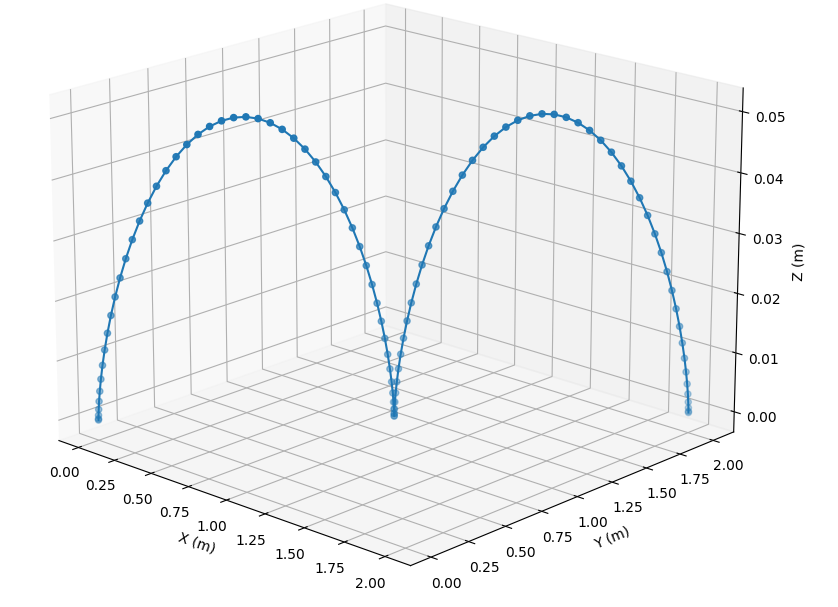
\includegraphics[width=1.0\textwidth]{Cycloid_space.png}
      \caption{Curva no espaço 3D.}
      \label{fig:traj_space}
    \end{subfigure}
    \begin{subfigure}[t]{0.32\textwidth}
      \centering
      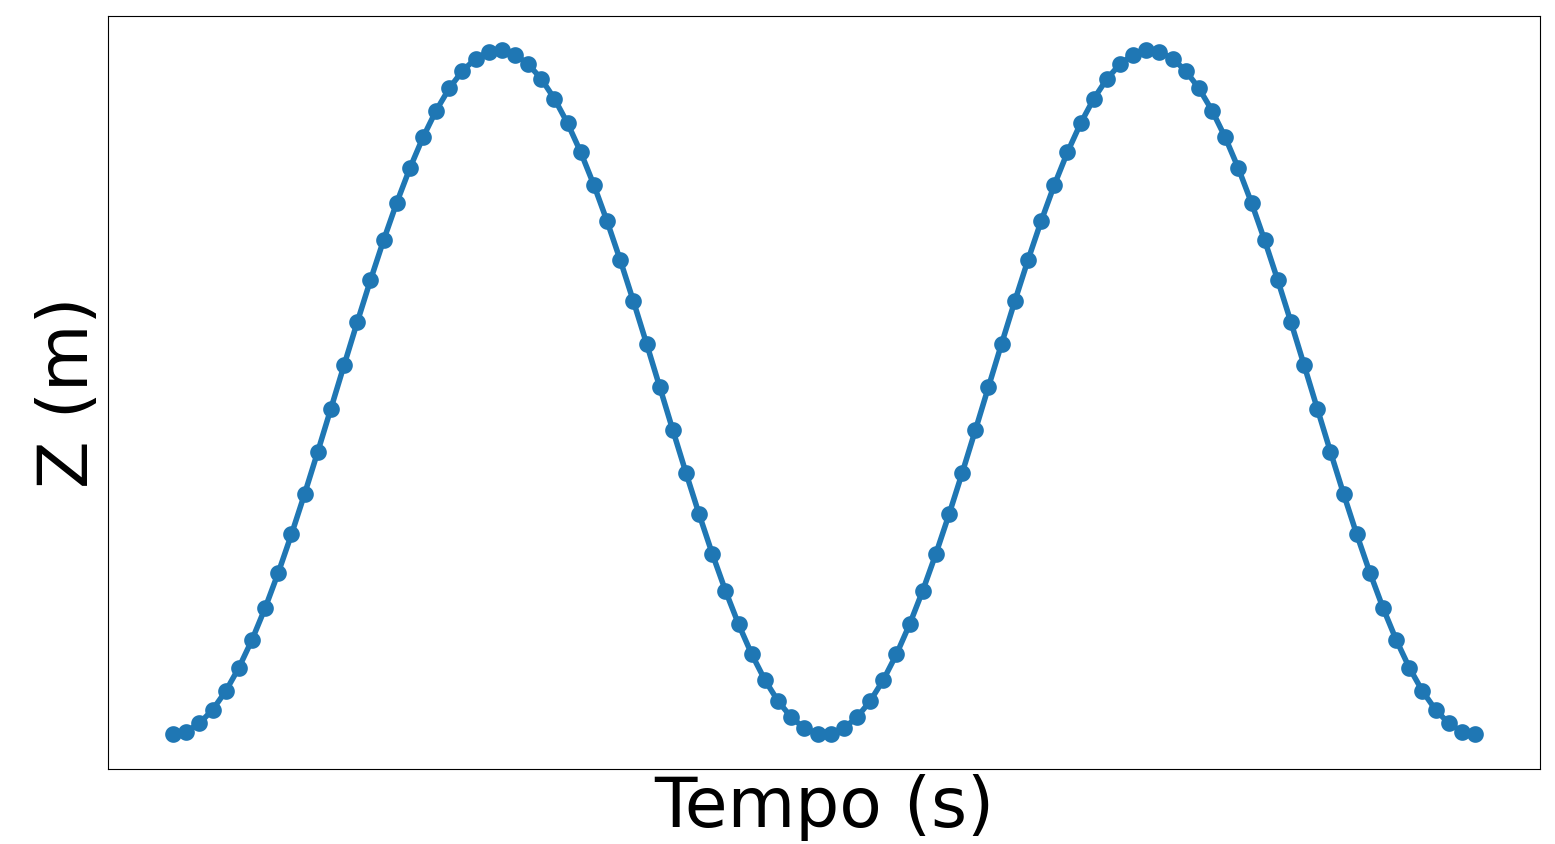
\includegraphics[width=1.0\textwidth]{Cycloid_time.png}
      \caption{Curva no tempo.}
      \label{fig:traj_time}
    \end{subfigure}
    \begin{subfigure}[t]{0.32\textwidth}
      \centering
      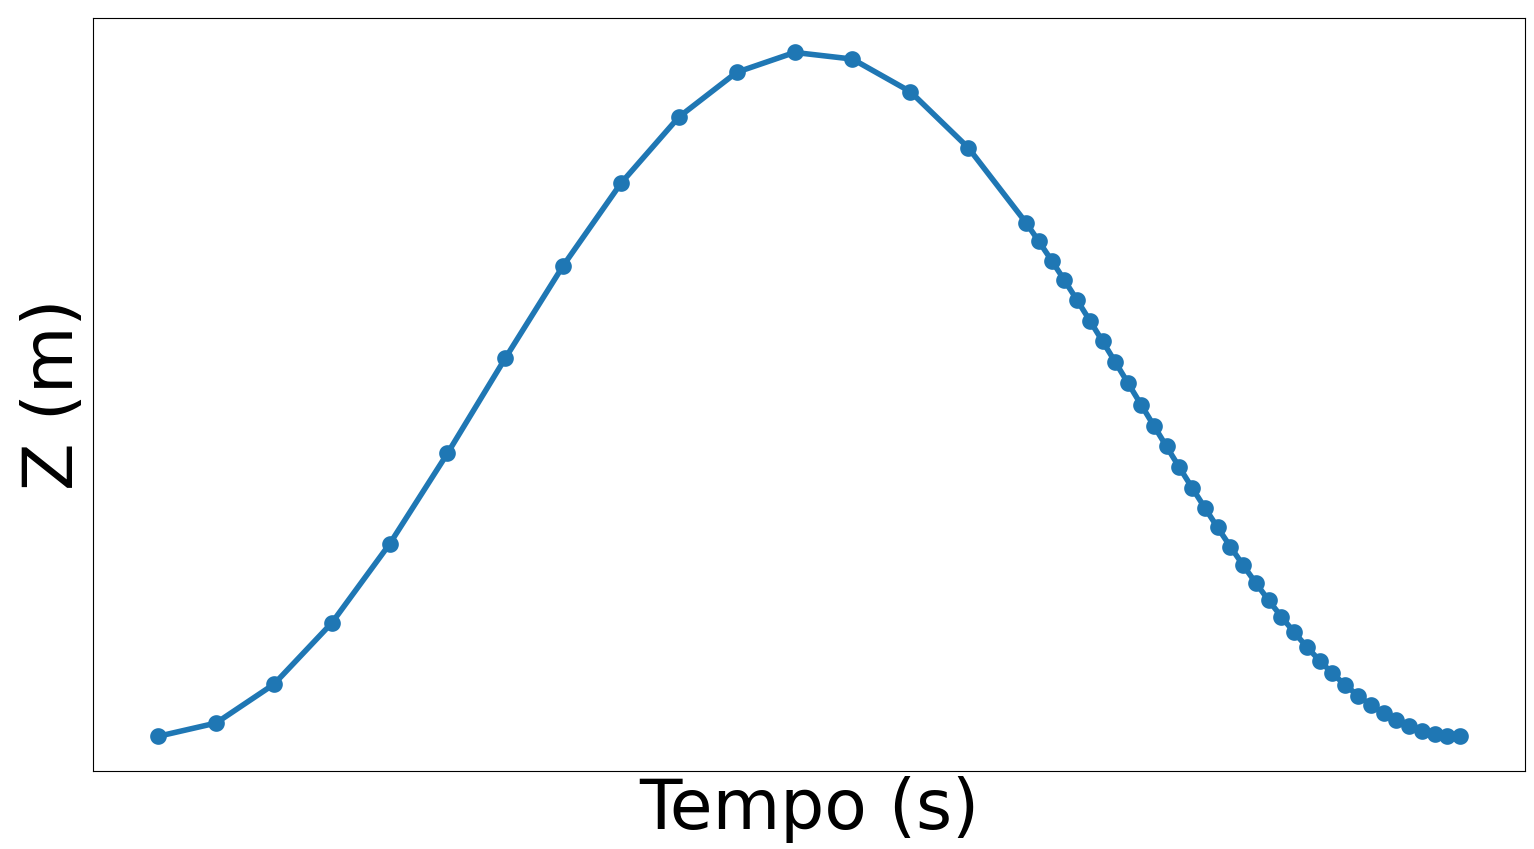
\includegraphics[width=1.0\textwidth]{Cycloid_modified.png}
      \caption{Curva com disposição de pontos modificada.}
      \label{fig:traj_time_modified}
    \end{subfigure}
    \vfill
    \caption{Trajetórias cicloidais para o passo de robô.}
    Fonte: autores.
    \label{fig:traj_curve}
\end{figure*}

Além da altura, distâncias em $x$ e $y$ e período, o planejador de trajetória do Caramelo também conta com dois parâmetros que têm como objetivo melhorar ainda mais o controle da força com que a pata toca o chão. Como os atuadores do robô são servomotores controlados por posição, o torque é proporcional ao deslocamento que este deve realizar entre os pontos da trajetória. Ou seja, quanto maior a resolução da trajetória, mais suave será o movimento. No entanto, a resolução da trajetória $N$ é fixa, dada em função do período do passo e da frequência de controle do planejador de marchas ($\SI{50}{\hertz}$) $N = 50T$. Logo, a estratégia adotada é a de espaçar a mesma quantidade de pontos de forma desigual ao longo do período do passo, de forma que haja mais pontos próximos ao momento em que a pata aterrissa no solo, e menos pontos próximos ao momento em que ela é erguida. O parâmetro $P_T$ é uma fração do período total do passo, e o parâmetro $P_N$, a fração do número total de pontos do passo que deve se encontrar entre o tempo $0$ e $P_T \cdot T$. Em outras palavras, se $P_T = 0,66$ e $P_N = 0,33$, $33\%$ de $N$ estará nos primeiros dois terços do período, enquanto os $67\%$ restantes estarão no um terço final. A trajetória, considerando esses parâmetros, está ilustrada na figura \ref{fig:traj_time_modified}.

\section{Resultados e Discussão}
A seguir, serão apresentados os resultados preliminares e os experimentos realizados com o Caramelo. 
  
  \subsection{Testes preliminares}
  \label{subsec:testes_preliminares}
  
  Os resultados preliminares referem-se aos resultados obtidos com as funcionalidades básicas do robô: capacidade de movimentação do corpo a partir do modelo cinemático, capacidade de controle da orientação do corpo com o controlador de angulação, e capacidade de seguir uma trajetória de passo calculada.

  No primeiro teste preliminar, foi avaliada a movimentação do corpo a partir do modelo cinemático. Foi observado que o sistema não só é capaz de realizar a cinemática de cada uma das pernas individualmente, como também do seu corpo em todos os 6 graus de liberdade (translações em $x$, $y$ e $z$ e rotações em $roll$, $pitch$ e $yaw$). A figura \ref{fig:moving_body} ilustra o movimento do corpo do robô em cada um desses graus de liberdade.

  \begin{figure}[!htb]
    \centering
    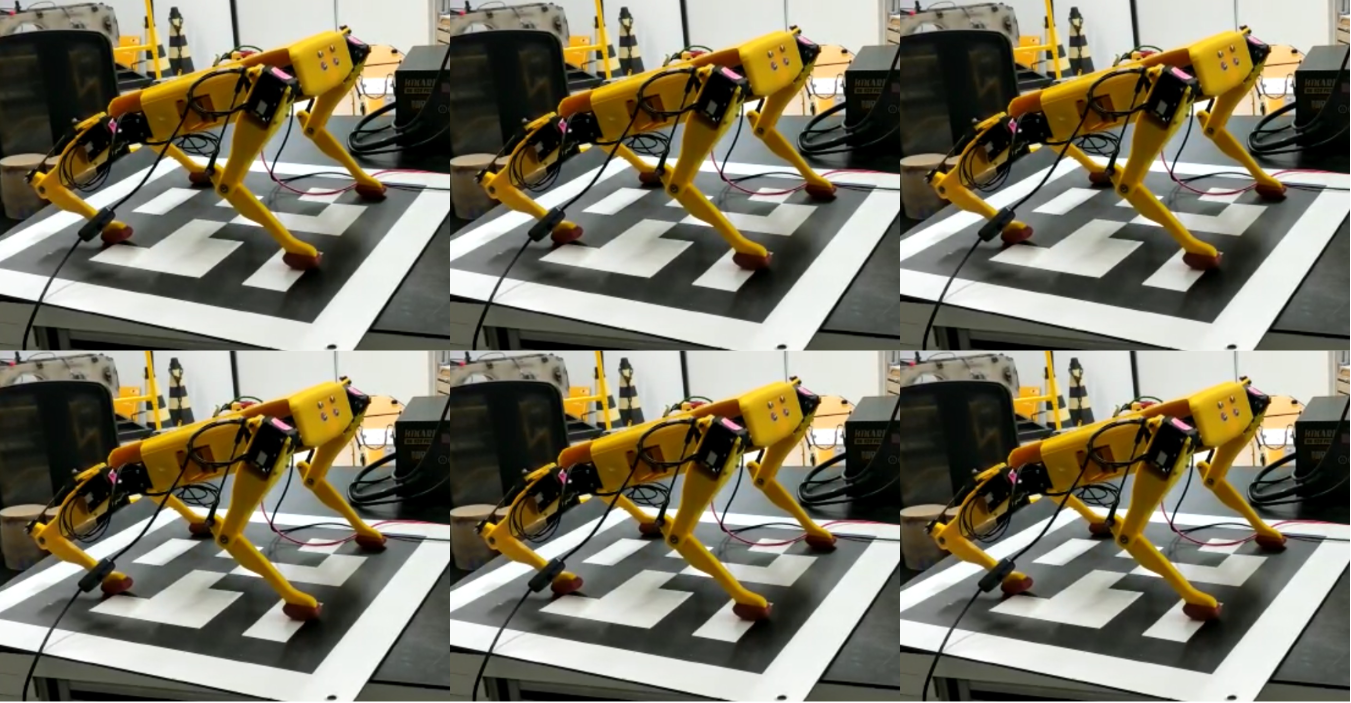
\includegraphics[width=0.48\textwidth]{moving_body.png}
    \caption{Movimentação do corpo do robô.}
    Fonte: autores.
    \label{fig:moving_body}
  \end{figure}

  A seguir, foi avaliada a performance do controlador de angulação do corpo. Os gráficos da figura \ref{fig:grafico_controlling} ilustram o comportamento do sistema à variação dos \textit{setpoints} de orientação em \textit{roll} e em \textit{pitch} para o corpo do robô ao longo do tempo. As curvas em azul representam os \textit{setpoints} aplicados como sinais degrau, enquanto que as curvas em vermelho ilustram o comportamento do sistema. Nota-se a capacidade que o protótipo tem de se adaptar rapidamente aos novos valores desejados de orientação em \textit{roll} e \textit{pitch}, simultaneamente.

  \begin{figure}
    \centering
    \begin{subfigure}[t]{0.48\textwidth}
      \centering
      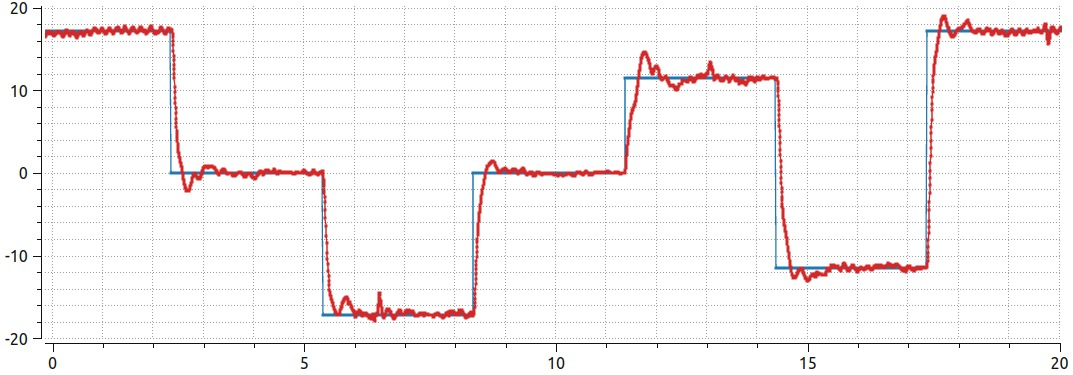
\includegraphics[width=1.0\textwidth]{grafico_controlling_X.png}
      \caption{\textit{Roll.}}
      \label{fig:controlling_roll}
    \end{subfigure}
    \begin{subfigure}[t]{0.48\textwidth}
      \centering
      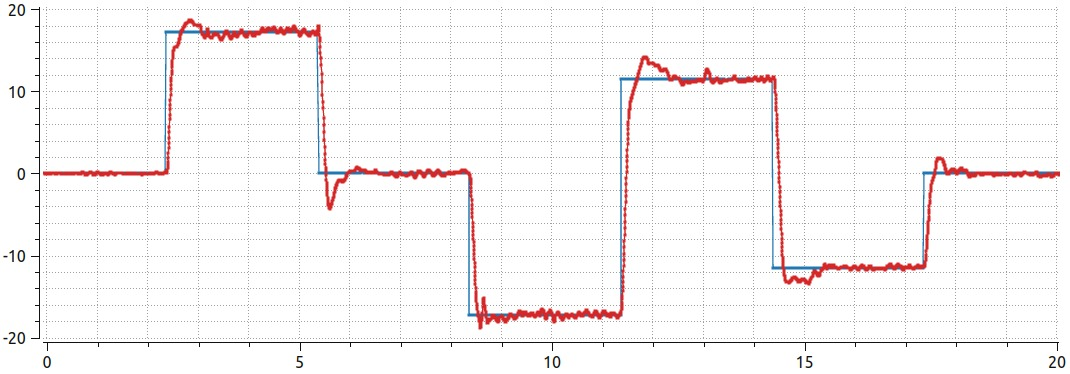
\includegraphics[width=1.0\textwidth]{grafico_controlling_Y.png}
      \caption{\textit{Pitch.}}
      \label{fig:controlling_pitch}
    \end{subfigure}
    \caption{Respostas dos controles de angulação.}
    Fonte: autores.
    \label{fig:grafico_controlling}
  \end{figure}

  O último teste preliminar teve o objetivo de analisar o tempo de execução da trajetória, as coordenadas finais $(x_{final}, y_{final})$ da pata e a altura máxima $z_{max}$ atingida durante o passo, comparando-os com os valores esperados para cada um desses parâmetros. A tabela \ref{tab:trajetoria} mostra as médias e desvios padrões encontradas para cada um desses parâmetros, durante a realização do teste.

  \begin{table}[!htb]
    \centering
    \begin{tabular}{ccc}
      \hline
      \textbf{Teste} & \textbf{1}      & \textbf{2}  \\
      \hline
      $\bar{tempo} (s)$         & 0,557  & 0,557 \\
      \hline
      $\sigma_{tempo} (s)$       & 0,008  & 0,008 \\
      \hline
      $\bar{x}_{final} (cm)$     & 5,034  & 3,024 \\
      \hline
      $\sigma_{x_{final}} (cm)$  & 0,009  & 0,013 \\
      \hline
      $\bar{y}_{final} (cm)$     & 2,924  & 4,915 \\      
      \hline
      $\sigma_{y_{final}} (cm)$  & 0,013  & 0,004 \\      
      \hline
      $\bar{z}_{max} (cm)$       & 4,760  & 4,755 \\      
      \hline
      $\sigma_{z_{max}} (cm)$    & 0,023  & 0,028 \\
      \hline   
    \end{tabular}

    \caption{Resultados dos teste da trajetória da pata.}
    Fonte: autores.
    \vspace{-\baselineskip}
    \label{tab:trajetoria}
  \end{table}
  

  Inicialmente, foram removidos os \textit{outliers} (valores do conjunto de dados acima ou abaixo dos limites superior e inferior, respectivamente) das amostras, valores que fogem da normalidade e podem prejudicar a análise dos dados. Em seguida, a fim de avaliar a normalidade dos dados, foram aplicados testes de Shapiro-Wilk nos dados de tempo e altura máxima de ambos os testes, os quais obtiveram $p_{valor} > 0,05$ em todos os casos. Isso indica que as amostras de ambos os testes estão semelhantes a uma distribuição normal para um nível de confiança de $95\%$. Posteriormente, foram realizados dois testes de análise de variância (ANOVA) unilaterais: o primeiro relacionando o tempo de execução da trajetória nos testes 1 e 2, e o segundo a altura máxima alcançada. O objetivo foi verificar se os resultados se alteraram para diferentes valores de $(x, y)$ requisitados. O resultado da ANOVA indica um $p_{valor}$ de aproximadamente $0,7212$ referente ao tempo, e de $0,5070$ referente à altura máxima alcançada durante o passo. Ambos os valores são superiores a $0,05$, indicando que não há uma diferença significativa entre as médias de cada teste, considerando um nível de confiança de $95\%$. Ou seja, diferentes pontos de destino em $(x, y)$ não interferiram no tempo de execução do passo, tampouco na altura máxima alcançada pela pata.

  O gráfico da figura \ref{fig:grafico_trajetoria_xyz} representa uma das amostras coletada para o primeiro teste ($x=0,05m$, $y=0,03m$), correspondente à trajetória em $z$ (altura do passo). Nota-se que, como esperado pela análise da tabela \ref{tab:trajetoria}, há um atraso na execução da trajetória (neste caso específico, de aproximadamente $54ms$), e a altura máxima alcançada é levemente inferior à desejada (alcançando, neste caso, um valor próximo a $0,0476m$).
  
  \begin{figure}[!htb]
    \centering
    % 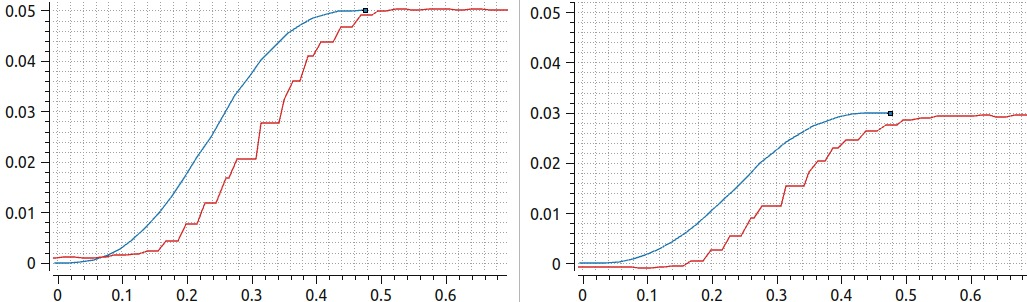
\includegraphics[width=0.48\textwidth]{grafico_trajetoria_xy.png}
    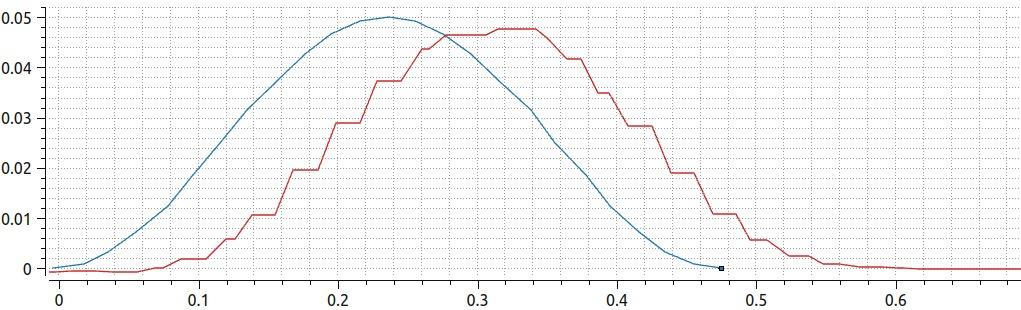
\includegraphics[width=0.48\textwidth]{grafico_trajetoria_z.png}
    \caption{Trajetórias realizadas pelas patas.}
    Fonte: autores.
    \label{fig:grafico_trajetoria_xyz}
  \end{figure}

  A distribuição das amostras de tempo e de altura máxima da pata em ambos os testes pode ser percebida pelos gráficos de \textit{box plot}, apresentados na figura \ref{fig:time_zmax_traj}. Nestes gráficos, é observado a proximidade entre as medianas dos testes e a similaridade na distribuição dos seus quartis, enfatizando a semelhança entre os resultados dos testes 1 e 2.

  \begin{figure}[!htb]
    \centering
    \caption{Tempo e altura da pata durante um passo.}
    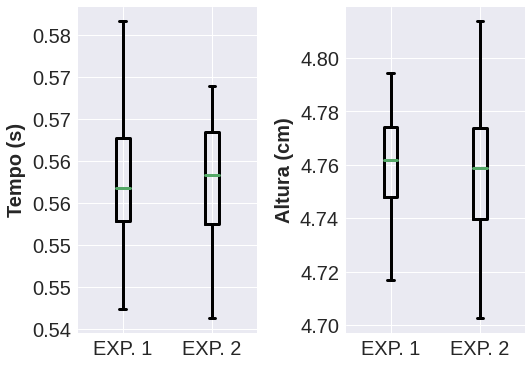
\includegraphics[width=0.48\textwidth]{tempo_zmax_traj.png}
    Fonte: autores.
    \label{fig:time_zmax_traj}
  \end{figure}

  \begin{figure}[!htb]
    \centering
    \begin{subfigure}[t]{0.49\textwidth}
      \centering
      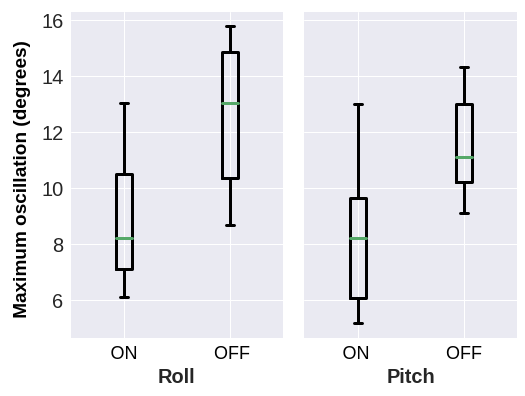
\includegraphics[width=1.0\textwidth]{plane_boxplot.png}
      \caption{Terreno plano.}
      \label{fig:imu_test_plane}
    \end{subfigure}
    \begin{subfigure}[t]{0.49\textwidth}
      \centering
      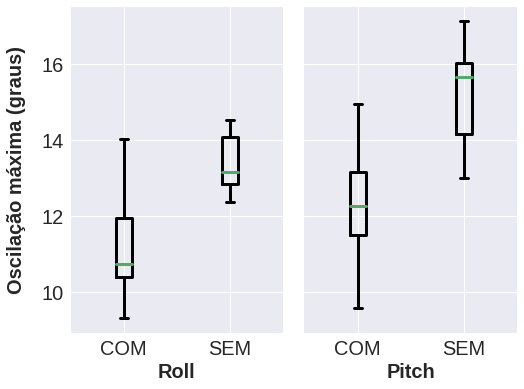
\includegraphics[width=1.0\textwidth]{irregular_boxplot.png}
      \caption{Terreno irregular.}
      \label{fig:imu_test_irregular}
    \end{subfigure}
    \caption{Oscilação do corpo em ambos os tipos de terreno.}
    Fonte: autores.
    \label{fig:imu_test}
  \end{figure}

  \subsection{Experimentos}
  A seguir, serão apresentados os resultados dos experimentos de locomoção descritos na seção \ref{sec:method_results_analysis}. Esses experimentos tiveram o objetivo de avaliar se o robô consegue se mover em uma velocidade desejada e o quão estável ele se mantém durante a caminhada. Foram coletados dados de velocidade média do robô (inferida com base no tempo que o robô levou para percorrer $1,5m$) e a oscilação máxima do corpo em \textit{roll} e \textit{pitch}. As médias e desvios padrões de cada variável para cada teste estão apresentadas na tabela \ref{tab:vel_stab}. 
  
  \begin{table}[!htb]
    \centering
    \begin{tabular}{ccccc}
      \hline
      \textbf{Teste} & \textbf{1} & \textbf{2} & \textbf{3} & \textbf{4} \\ \hline
      Ter. & Plano & Plano & Irreg. & Irreg. \\ \hline
      \begin{tabular}[c]{@{}c@{}}C. R.\end{tabular} & Não & Sim & Não & Sim \\ \hline
      \begin{tabular}[c]{@{}c@{}}Vel. \\ $(cm/s)$ \end{tabular} &   2,15   &  3,68  &   2,03  & 2,39  \\ \hline
      \begin{tabular}[c]{@{}c@{}} $\sigma_{Vel}$  \\ $(cm/s)$ \end{tabular} & 0,040 & 0,075 & 0,016 & 0,047 \\ \hline
      \begin{tabular}[c]{@{}c@{}} $\Delta_{Roll}$ \end{tabular} & 12,59\degree & 8,81\degree & 13,37\degree & 11,13\degree \\\hline
      \begin{tabular}[c]{@{}c@{}} $\sigma_{Roll}$ \end{tabular}  & 2,54\degree & 2,36\degree & 0,78\degree & 1,47\degree \\ \hline
      \begin{tabular}[c]{@{}c@{}} $\Delta_{Pitch}$ \end{tabular} & 11,55\degree & 8,31\degree & 15,19\degree & 12,09\degree \\ \hline
      \begin{tabular}[c]{@{}c@{}} $\sigma_{Pitch}$ \end{tabular}  & 1,89\degree & 2,63\degree & 1,44\degree & 1,66\degree \\ \hline

    \end{tabular}
    
    \caption{Resultados da análise da velocidade e estabilidade.}
    Fonte: autores.
    \label{tab:vel_stab}
  \end{table}

  A partir desses dados, foi observado que o robô não alcançou a velocidade desejada de $0,05 m/s$ em nenhum dos testes, alcançando apenas $74\%$ desse valor para a média de velocidades do teste feito em terreno plano com controle de estabilidade ativo. É possível justificar essa diferença pelo acúmulo de erros nas coordenadas finais $(x_f, y_f)$ das patas a cada passo, nesse cenário em que os atuadores do robô operam com carga. Isto é, ao operar sustentando o peso do robô, o sistema de controle não foi capaz de seguir fielmente a trajetória do passo, percorrendo com a pata uma distância menor do que a necessária para alcançar uma velocidade média de $0,05 m/s$. Esse resultado é diferente do que foi mostrado na seção \ref{subsec:testes_preliminares}, onde os motores foram avaliados em um cenário sem carga significativa.
  
  A tabela \ref{tab:vel_stab} também mostra que as oscilações médias em \textit{roll} e \textit{pitch} foram menores quando o controle de estabilidade estava ativo tanto no terreno plano quanto no irregular. A fim de comprovar que o controle de estabilidade contribuiu efetivamente para diminuir as oscilações do robô em ambos os tipos de terreno, o mesmo procedimento de análise do experimento anterior foi seguido. Primeiramente, foram removidos os \textit{outliers} das amostras e aplicado o teste de normalidade de Shapiro-Wilk, o qual indicou um $p_{valor} > 0,05$ para todos os casos. Em seguida, foi aplicado o teste ANOVA para comparar a oscilação em \textit{roll} e em \textit{pitch} dos testes 1 e 2. O mesmo processo foi repetido para os testes 3 e 4. O resultado da análise apontou que as distribuições de oscilação em \textit{roll} e \textit{pitch} são significativamente diferentes tanto no terreno plano quanto no terreno irregular, uma vez que o $p_{valor}$ de todos os testes foi inferior a $0,05$. Os gráficos da figura \ref{fig:imu_test} ilustram com mais detalhes a distribuição dos dados. Nota-se que com o controle de estabilidade, a oscilação foi mais dispersa na maioria dos testes, o que pode ser comprovado analisando os desvios padrões apresentados na tabela \ref{tab:vel_stab}. No entanto, exceto quanto à oscilação em \textit{roll} no terreno plano, o terceiro quartil está abaixo do primeiro quartil das distribuições de oscilação sem o controle de estabilidade, mostrando que o controlador diminuiu a oscilação do corpo do robô em \textit{roll} ou em \textit{pitch} em pelo menos $75\%$ das amostras coletadas.


\section{Conclusão}

Este trabalho abordou os conceitos utilizados para locomoção de robôs quadrúpedes e buscou aplicá-los no desenvolvimento de um robô real. O Caramelo foi desenvolvido para fins de educação e pesquisa na área de robôs com pernas, mais especificamente quadrúpedes. Trata-se de um projeto \textit{open source}, cujo código fonte está disponível publicamente no \textit{GitHub} \cite{CaramelRepo}. 
  
Os testes e experimentos realizados buscaram avaliar a performance da locomoção do robô no espaço tridimensional. Os testes preliminares indicaram que o robô possui a capacidade de mover o corpo em 6 GDL e controlar sua orientação em $roll$ e $pitch$. Além disso, pôde-se concluir que a pata é capaz de seguir uma trajetória até um ponto requisitado em $x$ e $y$ no cenário sem carga. Não foram constatadas diferenças significativas no tempo total e na altura máxima da trajetória nos dois testes realizados. Contudo, foi observado um atraso no tempo de execução trajetória, relacionado ao atraso na resposta dos motores.
 
Os experimentos de locomoção mostraram que o robô não alcançou a velocidade desejada em nenhum dos testes, estando  a velocidade média do teste no terreno plano com o controle de angulação ativo a mais próxima deste valor. Essa diferença pode estar relacionada com o fato de que o sistema de controle não conseguiu operar de forma adequada quando sustentando o peso do robô. Como o controle da trajetória é feito em malha aberta (apenas os controladores individuais das juntas possuem malha fechada), não há compensação, e a pata não alcança a distância esperada. Ademais, também pôde-se observar que o controle de angulação resultou numa maior estabilidade do robô em ambos os terrenos.

\section{Considerações Finais}

Para trabalhos futuros, recomenda-se a revisão dos atuadores usados no robô. Ao longo da fase de testes, foi observado que estes frequentemente falhavam por conta de sobrecarga, o que é um sinal de que foram subdimensionados. Por consequência, a capacidade de \textit{payload} não é significativa. Uma possível solução para essa questão é a substituição do modelo atual por um com maior torque e/ou a investigação da configuração das pernas do robô. A equipe observou que, como os motores que mais falhavam eram os traseiros, adotar a configuração \textit{elbow-knee} pode diminuir a carga neles, já que deixaria as pernas traseira em uma configuração simétrica às frontais. Espera-se, também, que isso influencie na performance de locomoção, deixando o robô mais rápido e estável. Além disso, sugere-se a aplicação de outros métodos de controle, como controladores baseados em modelos dinâmicos ou até em \textit{machine learning}.


\section*{Acknowledgment}

The preferred spelling of the word ``acknowledgment'' in America is without 
an ``e'' after the ``g''. Avoid the stilted expression ``one of us (R. B. 
G.) thanks $\ldots$''. Instead, try ``R. B. G. thanks$\ldots$''. Put sponsor 
acknowledgments in the unnumbered footnote on the first page.

\section*{References}

Please number citations consecutively within brackets \cite{b1}. The 
sentence punctuation follows the bracket \cite{b2}. Refer simply to the reference 
number, as in \cite{b3}---do not use ``Ref. \cite{b3}'' or ``reference \cite{b3}'' except at 
the beginning of a sentence: ``Reference \cite{b3} was the first $\ldots$''

Number footnotes separately in superscripts. Place the actual footnote at 
the bottom of the column in which it was cited. Do not put footnotes in the 
abstract or reference list. Use letters for table footnotes.

Unless there are six authors or more give all authors' names; do not use 
``et al.''. Papers that have not been published, even if they have been 
submitted for publication, should be cited as ``unpublished'' \cite{b4}. Papers 
that have been accepted for publication should be cited as ``in press'' \cite{b5}. 
Capitalize only the first word in a paper title, except for proper nouns and 
element symbols.

For papers published in translation journals, please give the English 
citation first, followed by the original foreign-language citation \cite{b6}.

\begin{thebibliography}{00}
\bibitem{b1} G. Eason, B. Noble, and I. N. Sneddon, ``On certain integrals of Lipschitz-Hankel type involving products of Bessel functions,'' Phil. Trans. Roy. Soc. London, vol. A247, pp. 529--551, April 1955.
\bibitem{b2} J. Clerk Maxwell, A Treatise on Electricity and Magnetism, 3rd ed., vol. 2. Oxford: Clarendon, 1892, pp.68--73.
\bibitem{b3} I. S. Jacobs and C. P. Bean, ``Fine particles, thin films and exchange anisotropy,'' in Magnetism, vol. III, G. T. Rado and H. Suhl, Eds. New York: Academic, 1963, pp. 271--350.
\bibitem{b4} K. Elissa, ``Title of paper if known,'' unpublished.
\bibitem{b5} R. Nicole, ``Title of paper with only first word capitalized,'' J. Name Stand. Abbrev., in press.
\bibitem{b6} Y. Yorozu, M. Hirano, K. Oka, and Y. Tagawa, ``Electron spectroscopy studies on magneto-optical media and plastic substrate interface,'' IEEE Transl. J. Magn. Japan, vol. 2, pp. 740--741, August 1987 [Digests 9th Annual Conf. Magnetics Japan, p. 301, 1982].
\bibitem{b7} M. Young, The Technical Writer's Handbook. Mill Valley, CA: University Science, 1989.
\end{thebibliography}
\vspace{12pt}
\color{red}
IEEE conference templates contain guidance text for composing and formatting conference papers. Please ensure that all template text is removed from your conference paper prior to submission to the conference. Failure to remove the template text from your paper may result in your paper not being published.

\end{document}
